\subsection{05.04.19}
\subsubsection{Паросочетания}
Граф $G$ называется двудольным, если: $V(G) = V_1 \cup V_2, V_1 \cap V_2 = \varnothing, V_1, V_2 \neq \varnothing, \forall e = uv \in E(G): u \in V_1, v \in V_2$.\\
Полный двудольный граф - двудольный граф, в котором $\forall u \in V_1, v \in V_2: uv \in E(G)$.\\
Будем называть $V_1$ множеством начал, а $V_2$ множеством концов двудольного графа.\\
Паросочетание - множество $M \subseteq E(G)$ такое что: $\forall e_1 \neq e_2 \in M: e_1 \cap e_2 = \varnothing$.\\
Будем называть $I \subseteq V_1$ множеством начал, $J \subseteq V_2$ множеством концов ребер паросочетания $M$ на двудольном графе.\\
Тогда $M$ можно задать биекцией $\phi: I \rightarrow J$ такой что $ \phi(i) = j \Longleftrightarrow ij \in M$.\\
Максимальным паросочетанием называется максимальное по включению паросочетание.\\
\begin{figure}[h]
        \center{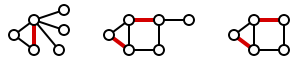
\includegraphics{Maximal-matching.png}}
    \caption{Примеры максимальных паросочетаний}
    \label{fig:Maximal-matching}
\end{figure}\\
Наибольшим паросочетанием называется наибольшее по мощности максимальное паросочетание.\\
\begin{figure}[h]
        \center{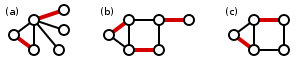
\includegraphics{Maximum-matching.png}}
    \caption{Примеры наибольших паросочетаний}
    \label{fig:Maximum-matching}
\end{figure}\\
Совершенным паросочетанием называется паросочетание, в котором каждая вершина инцидента какому-то ребру паросочетания.\\
Задача: построить наибольшее паросочетание на произвольном двудольном графе $G$.\\
$C \subseteq V(G)$ называют контролирующим множеством, если $\forall e \in E(G): C \cap e \neq \varnothing$.\\
Двойственная задача: построить минимальное контролирующее множество на произвольном двудольном графе $G$.\\
\underline{\bfЛемма}: Размер любого паросочетания не больше размера любого контролирующего множества.\\
\underline{\bfДоказательство}: Пусть $M$ - паросочетание и существует контролирующее множество $C$ такое что $|M| \textless |C| \Rightarrow \exists u \in C: \exists e_1 \neq e_2 \in M: e_1 \cap e_2 = u \Rightarrow e_1 \cap e_2 \neq \varnothing \Rightarrow$ противоречие с определением паросочетания $\Rightarrow |M| \leq |C|$.\\
\begin{figure}[h]
        \center{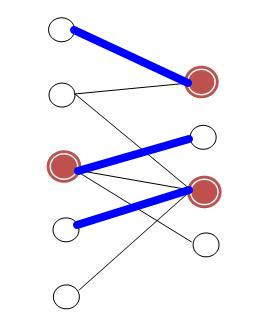
\includegraphics{Minimal-Cover.jpg}}
    \caption{Синее - максимальное паросочетание, красное - минимальное контролирующее множество}
    \label{fig:Maximal-matching and minimal-cover}
\end{figure}\\\\\\\\
\underline{\bfТеорема}: Размер наибольшего паросочетания равен размеру наименьшего контролирующего множества.\\
\underline{\bfДоказательство}: Исходя из леммы: размер наибольшего паросочетания не больше размера наименьшего контролирующего множества. Будем строить по индукции паросочетание и контролирующее его множество. $M_0 = \varnothing, C_0 = \varnothing$ - база. Пусть построено некоторое паросочетание $M_n$ на двудольном графе $G$ и множество $C_n \subseteq V(G)$ такое что $C_n$ контролирует все ребра $M_n$ и $|M_n| = |C_n|$. Если $C_n$ - контролирующее множество, то все доказано. Пусть $\exists e = uv (u \in V_1, v \in V_2)$ такое что $e \cap C_n = \varnothing$.\\
Случай 1: $\forall e' \in M: e' \cap \{u, v\} = \varnothing$. Тогда $M_{n + 1} = M_n \cup {e}, C_{n + 1} = V_1 \cap V(M_{n + 1})$.\\
Случай 2: $\exists e' \in M: e' \cap \{v\} \neq \varnothing, \forall e'' \in M: e'' \cap \{u\} = \varnothing$. Тогда определим дублера для $e': \delta(e') = e, rank(e') = rank(e) = 1$ и $M_{n + 1} = M_n, C_{n + 1} = C_n \setminus \{V_1 \cap e'\} \cup \{v\}$.\\
Случай 3: $\exists e' \in M: e' \cap \{v\} \neq \varnothing, \exists e'' \in M: e'' \cap \{u\} \neq \varnothing, rank(e'') = k$. Тогда $\delta(e') = e, rank(e') = rank(e) = k + 1$ и $M_{n + 1} = M_n, C_{n + 1} = C_n \setminus \{V_1 \cap e'\} \cup \{v\}$.\\
Случай 4: $\exists e''_k \in M: e''_k \cap \{u\} \neq \varnothing, \forall e' \in M: e' \cap \{v\} = \varnothing, rank(e''_k = k), \exists e''_{k - 1}, ..., e''_1 \in M: rank(e''_i) = i$ $ \forall i \in 1:k, \forall i \in 2:k:$ $V_1 \cap \delta(e''_i) = V_1 \cap e''_{i - 1}$. Тогда $M_{n + 1} = M_n \setminus \{e'_1, ..., e'_k\} \cup \{\delta(e'_1, ..., \delta(e'_k), e\}, C_{n + 1} = V_1 \cap V(M_{n + 1})$ и $\forall e \in E(G): rank(e) = 0, \delta(e) = \varnothing$.\\
Таким образом $|M_{n + 1}|\geq |M_n|, |C_{n + 1}| = |M_{n + 1}|$ и $C_{n + 1}$ контролирует $M_{n + 1}$.\\
В результате работы алгоритма будет построено наибольшее паросочетание $M_m$ и равное ему по размеру контролирующее множество $C_m$.\\
Примечание: не знаю насколько это неочевидно, но вот почему $C_m$ наименьшее контролирующее множество: Пусть $\exists C_{m'}: |C_{m'}| < |C_m|$ и $C_{m'}$ контролирующее множество. Тогда $|M_m| = |C_m| > |C_{m'}|$ что противоречит лемме.
